\part{Diseño}\label{part:diseno}

\section{Hardware}\label{sec:hw}
\subsection{Diagrama en bloques general}
El sistema se compone de módulos que interactúan entre sí, intercambiando datos entre ellos. En primer lugar el maestro, es el encargado de recibir los datos que el cliente le proporciona. Es el que posee el microcontrolador que comanda todo el sistema (ver figura \ref{fig:dibujo-real}).

Por otra parte los esclavos obtienen la información que les transmite el microcontrolador y actualizan la matriz de LEDs que tienen asociada. En la figura \ref{fig:diagrama-bloques-general} se puede observar un diagrama en bloques de todo el sistema.

\begin{figure}[!ht]
	\centering
	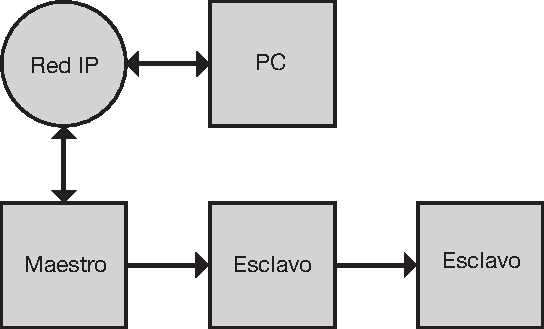
\includegraphics[scale=1]{imagenes/esquema-general.pdf}
	\caption{Esquema general entre todos los componentes del sistema.}
	\label{fig:diagrama-bloques-general}
\end{figure}

En la figura \ref{fig:diagrama-bloques-general}, leyendo de izquierda a derecha, se observa en primer lugar un cliente. Ésto se representa a través de una aplicación de PC, siendo ésta, una de las formas que el cliente tiene para interactuar con el sistema.

Conectando su computadora a la misma red que se encuentra vinculado el cartel, el cliente puede, por medio de dicha aplicación, enviar los comandos para que el sistema satisfaga sus necesidades.

Por medio del protocolo de comunicación WiFi, los datos llegan hacia el microcontrolador que se encuentra en el módulo maestro. Cabe destacar que el protocolo de red que encapsula las distintas acciones que el usuario puede realizar ha sido diseñado completamente para este proyecto y se explica en mayor detalle en el apéndice \ref{sec:protocolo}.
Dicho protocolo se implementa tanto del lado de la aplicación de PC, como del microcontrolador que controla el cartel.

Tras recibir y decifrar los datos, el microcontrolador procesa la información y la transmite vía protocolo serie, sincrónico hacia el primer driver MAX7219 que controla la primera matriz de LEDs.

Resulta necesario aclarar que cada módulo esclavo posee un MAX7219 y la información que le proporciona el microcontrolador se transmite sólo al primerero de ellos. Luego la misma se desplaza entre los diferentes MAX7219 utilizando determinados pines de dicho módulo.
De esta forma, el microcontrolador solo mantiene una conexión física directa con el primer driver.

Finalmente, cada módulo esclavo enciende en su respectiva matriz de LEDs, la información suministrada por el maestro, de forma de mostrar el mensaje que el cliente había enviado inicialmente por medio de la aplicación de PC.

Cabe destacar que la comunicación entre la aplicación de PC y el cartel es bidireccional, debido a que todas las operaciones que el cliente realice, necesitan de una respuesta.
En algunos casos, dicha respuesta es solo para indicar éxito o error, mientras que en otros casos el usuario recibe parámetros de configuración y las credenciales de red a las que el sistema se encuentra actualmente conectado.

\subsection{Fuente de alimentación}
El cartel requiere una alimentación de 5V de corriente continua. Para esto se expone un conector hembra (de 5.5mm x 2.1mm), el cual se conecta a un transformador externo de 220V AC a 5V DC. El sistema no posee batería de ningún tipo.
%TODO AMG - falta poner análisis de consumo. Todo lo que se hizo, incluso lo que después se descartó.

\subsection{Módulo maestro}
Como se mencionó anteriormente, este módulo se encarga de procesar los datos enviados desde el cliente y controlar los módulos esclavos que componen el cartel. Este módulo maestro almacena los parámetros de configuración previamente establecidos desde la aplicación de PC. Uno de ellos es la red WiFi a la que debe conectarse. Para evitar que el cartel sea inaccesible por una mala configuración accidental de la red, se añadió el diseño un pulsador de RESET, el cual, al ser presionado durante 5 segundos, reestablece los parámetros de configuración por defecto y reinicia el módulo maestro.

Por otro lado, resulta necesario comunicar al firmware del microcontrolador la cantidad de carteles que conforman el eslabón de esclavos. Para esto se utiliza un conjunto de jumpers que codifican la cantidad de carteles conectados, de manera que el usuario pueda agregar o quitar carteles sin necesidad de volver a cargar el firmware modificado. Ésto se explica en mayor detalle en el manual de usuario (ver sección \ref{sec:manual-usuario}).

\subsubsection{Microcontrolador}
El componente central en el módulo maestro es el microcontrolador ESP8266EX (figura \ref{fig:esp8266ex}), el cual se encuentra contenido en un módulo AI-Thinker ESP-12E (figura \ref{fig:foto-esp12e}), el cual está montado sobre un módulo NodeMCU que le provee de regulación de tensión y un conversor de serie TTL a USB. El ESP8266EX es un SoC (\emph{System on Chip}) de la empresa Espressif. El módulo NodeMCU es hardware libre, sin embargo, el ESP12E y el ESP8266EX no lo son.\cite{NodeMCU}

Es importante tener en cuenta que el sistema no integra en su hardware directamente ni el ESP12E ni el ESP8266EX, sino que utiliza el NodeMCU, cuya asignación de pines se puede ver en la figura \ref{fig:nodemcu-pinout}.

\begin{figure}[ht!]
	\begin{center}
		\includegraphics[width=8cm]{imagenes/esp12e-foto.jpg}
		\caption{Foto del módulo ESP12E sin su cubrimiento.}
		\label{fig:foto-esp12e}
	\end{center}
\end{figure}

\begin{figure}[ht!]
	\begin{center}
		\includegraphics[width=3cm]{imagenes/esp8266ex.jpg}
		\caption{Foto del integrado ESP8266EX.}
		\label{fig:esp8266ex}
	\end{center}
\end{figure}

\begin{figure}[ht!]
	\begin{center}
		\includegraphics[width=0.95\textwidth]{imagenes/nodemcu-pinout.pdf}
		\caption{Asignación de pines del NodeMCU.}
		\label{fig:nodemcu-pinout}
	\end{center}
\end{figure}

El chip ESP8266EX combina un microcontrolador Tensillica Xtensa L106, un RISC de 32 bits corriendo a 80 Mhz, con funcionalidad WiFi. \cite{ESP8266Datasheet} El chip tiene memoria ROM con firmware no removible, y puede correr programas almacenados en flash externa. Para poder usar todas sus funcionalidades, se debe programar sobre firmware privativo desarrollado por Espressif, esto implica que el programa de usuario corre en simultáneo con el firmware (utilizando funciones disponibilizadas por el firmware) y el uso de la memoria de trabajo está sujeto a la versión del firmware. Según el datasheet del ESP8266EX, el usuario puede esperar tener disponible 50 KiB de RAM para alocar variables globales o utilizando la heap.

El firmware de Espressif para el ESP8266EX implementa por completo la pila de protocolos TCP/IP, el protocolo 802.11 b/g/n/e/i y Wi-Fi Direct.

El ESP8266EX está diseñado con tecnologías de manejo de consumo y está dirigida a dispositivos móviles, dispositivos \emph{wearables} y para aplicaciones de internet de las cosas (IoT).

El hardware del microcontrolador opera en tres modos: modo activo, \emph{sleep} y \emph{deep-sleep}. Sin embargo, para este proyecto en particular, donde el dispositivo no tiene batería y está conectado permanentemente a la red eléctrica, no se utiliza ningún modo aparte del activo.

El microcontrolador provee 17 pines GPIO. El firmware permite emular mediante \emph{bit-banging} los protocolos SPI, SDIO, I2C, I2S y UART en cualquier pin que el programador elija y esté disponible para su uso. No todos los pines pueden ser utilizados libremente, ya que algunos de ellos están conectados a la memoria flash. El firmware también incluye una implementación software de PWM, ya que el microcontrolador no posee hardware de PWM real.

Se puede ver un diagrama de bloques del ESP8266EX en la figura \ref{fig:diagrama-bloques-esp8266ex}.

\begin{figure}[htp!]
	\centering
	\begin{center}
	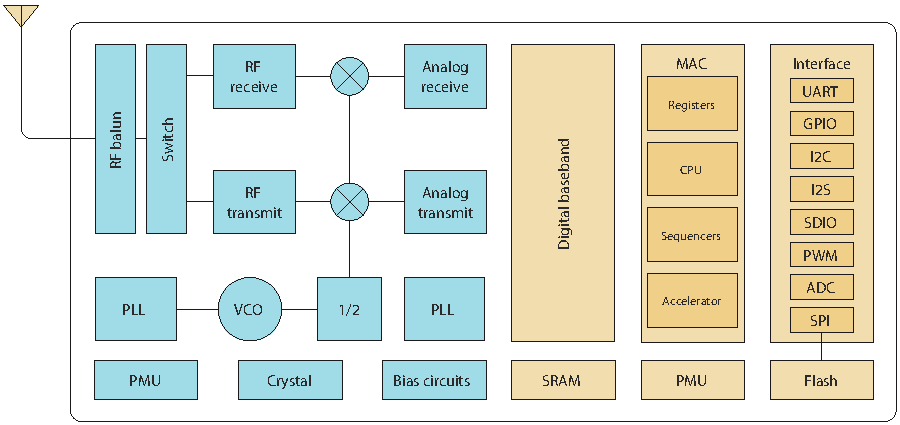
\includegraphics[width=\linewidth]{imagenes/diagrama-bloques-esp8266.pdf}
	\caption{Diagrama de bloques del Espressif ESP8266EX.}
	\label{fig:diagrama-bloques-esp8266ex}
	\end{center}
\end{figure}

Como se mencionó anteriormente, se necesita de flash externa para correr programas. El módulo ESP-12S se encarga de proveer al ESP8266EX 4 MiB de memoria flash.

\subsection{Módulo esclavo}
Un modulo esclavo posee un driver MAX7219, que es el componente principal junto con una interfaz que permite conectarse a otro módulo esclavo o en su defecto al master.

\subsubsection{MAX7219}\label{sec:max7219}
El MAX7219 es un controlador compacto, de entrada y salida en serie de cátodo común que conectan, indirectamente, microcontroladores a LEDs numéricos de siete segmentos de hasta ocho dígitos, pantallas de gráfico de barras o, en este caso, 64 LED individuales dispuestos de forma matricial. Se incluye en el chip, un decodificador BCD, circuitos de multiplexación, controladores de segmentos y dígitos, y una RAM estática de 8x8 que almacena cada número, o en este caso, mapas de bits. Solo se necesita una resistencia externa para configurar la corriente para todos los LEDs.

Las matrices individuales se pueden actualizar sin reescribir toda la pantalla.

Su alimentación V\texttt{+} debe estar entre 4 y 5.5 Volts para su correcto funcionamiento. En cambio los voltaje de las entradas lógicas tienen una restricción de que un valor alto como mínimo debe ser 3.5V y un valor bajo debe ser como máximo 0.8V.

Las características principales que posee el chip integrado se enumeran a continuación:
\begin{itemize}
	\item Interfaz serie de 10 MHz.
	\item Control de segmento LED individual.
	\item Selección de dígitos Decode / No-Decode.
	\item Apagado de baja potencia de 150 microA (datos retenidos).
	\item Control de brillo digital y analógico.
	\item Pantalla borrada al encenderse.
	\item Unidad de visualización LED de cátodo común.
	\item SPI, QSPI, interfaz serie Microwire paquetes DIP y SO de 24 pines.
\end{itemize}

La disposición de los pines del MAX7219 se puede observar en la figura \ref{fig:MAX-pines} y la descripción de cada uno en la tabla \ref{table:MAX-pines}.

Es necesario prestar atención en el conexionado con respecto a los pines de tierra (GND) ya que ambos deben estar conectados para el driver pueda funcionar correctamente, ambas estan al lado izquierdo de la figura \ref{fig:MAX-pines} (Pin 4 y 9).

Por otro lado, el MAX7219 tiene un pin denominado DOUT (pin 24) se utiliza para encadenar varios MAX7219 y de esta forma pasar la información al que esta directamente conectado, éste pin nunca tiene alta impedancia.

\begin{figure}[htp!]
	\centering
	\begin{center}
	\includegraphics[scale=1.2]{imagenes/hw/max.pdf}
	 \caption{Configuración de pines del chip MAX7219.}
	  \label{fig:MAX-pines}
	\end{center}
\end{figure}

\begin{table}[htp!]
\centering
\caption{Descripción de los pines del MAX7219}
\label{table:MAX-pines}
\begin{tabular}{C{10mm} C{14mm} L{108mm}}
\hline
Pin               & Nombre          & Función    \\ \hline
1                 & DIN             & Pin de datos seriales. Los datos son cargados en el registro de 16 bits en cada flanco ascendente del clock. \\
2, 3, 5–8, 10, 11 & DIG 0 - DIG 7    & Líneas de transmisión de ocho dígitos que absorben corriente del cátodo común de la pantalla. El MAX7219 deja en V+ cuando esta apagado. Los dígitos están en alta impedancia cunado se apaga.\\
4, 9              & GND             & Tierra.\\
12                & LOAD            & Pin de control. Los últimos 16 bits del Serial Data son cargados en el flanco ascendente. \\
13                & CLK             & Pin de clock serial. En cada flanco ascendente, los datos sin shifteados dentro de un registro interno. En cada flanco descendente los datos salen de DOUT. En el MAX7221, la entrada CLK está activa solo mientras LOAD está baja. \\
14–17, 20-23      & SEG A–SEG G, DP & Las unidades de siete segmentos y el punto decimal impulsan la fuente de corriente a la pantalla. Cuando un controlador de segmento está apagado, se conecta a GND.\\
18                & ISET            & Conectar a  $V_{DD}$ a través de una resistencia ($R_{SET}$) para configurar la corriente que pueda entregar a los dígitos y segmentos. \\
19                & V+              & Fuente positiva de corriente, conectar a 5 V. \\
24                & DOUT            & Salida de datos en serie. Los datos en DIN son válidos en DOUT 16.5 ciclos de reloj más tarde. \\ \hline
\end{tabular}
\end{table}

\begin{figure}[htp!]
\centering
\begin{center}
	\includegraphics[width=0.8\textwidth]{imagenes/hw/conexion-MAX-matriz.pdf}
	\caption{Conexión entre MAX7219 y su módulo de LEDs.}
	\label{fig:MAX-matriz}
\end{center}
\end{figure}

\begin{figure}[htp!]
\centering
\begin{center}
	\includegraphics[width=0.7\textwidth]{imagenes/hw/conexion-MAX-matriz.JPG}
	\caption{Fotografía de conexión entre MAX7219 y su módulo de LEDs.}
	\label{fig:MAX-matriz-real}
\end{center}
\end{figure}


\subsection{Matriz de LEDs}
La matriz posee 64 LEDs organizados en ocho filas y ocho columnas, con cátodo común en las columnas como se observa en la figura \ref{fig:modulo-led}. Se analizaron las dimensiones más apropiadas para la utilidad del cartel y se llegó a una separación de 12mm entre LEDs la cual mantiene un dpi apropiado (consiguiendo verse las letras a 10 metros), las demás medidas de pueden observar en la figura \ref{fig:modulo-led-dimensiones}.

Cada uno de los MAX7219 está conectado a una matriz, sus conexiones se pueden observar en el diagrama \ref{fig:MAX-matriz}. Adicionalmente, en la figura \ref{fig:MAX-matriz-real} se observa el prototipo que complementa el esquema de conexión de la figura previamente mencionada.

A la hora de efectuar las conexiones, se debe prestar principal atención a la orientación de la matriz. En la figura \ref{fig:MAX-matriz-real} se indica claramente cuáles son las filas (y su orden) y cuáles son las columnas. Con dicha información el proceso de conexionado se simplifica.

\begin{figure}[!htp]
	\centering
	\includegraphics[width=0.7\linewidth]{imagenes/hw/modulo-led.pdf}
	\caption{Esquema de conexiones de la matriz de LEDs.}
	\label{fig:modulo-led}
\end{figure}
\begin{figure}[!htp]
	\centering
	\includegraphics[width=\linewidth]{imagenes/hw/modulo-led-dimensiones.pdf}
	\caption{Dimensiones de la matriz de LEDs.}
	\label{fig:modulo-led-dimensiones}
\end{figure}


\subsection{Comunicación entre los módulos}
Para la comunicación maestro-esclavo y esclavo-esclavo se utiliza un protocolo serie de un bit sincrónico. Cada módulo esclavo tiene en su MAX7219 una entrada de serie junto a un clock, de manera que se toma el valor del bit en el flanco ascendente del reloj. A su vez, cada MAX7219 tiene un registro de desplazamiento de 16 bits, que en cada flanco ascendente del clock inserta en orden FIFO al registro un bit (DIN) y, en el flanco descendente del reloj, coloca en su salida el valor del bit más viejo en el registro de desplazamiento (DOUT). Por último, el MAX7219 tiene una entrada llamada LATCH que al pasar a alto, provoca que el MAX7219 \enquote{tome} la palabra de 16 bits, interpretándola como se describió en la sección \ref{sec:max7219}.

De esta manera es posible dirigir una palabra arbitraria a cualquier esclavo, y es particularmente eficiente en el caso en que se debe mandar una palabra a cada MAX7219 y se desea que todas la interpreten a la vez. Es cuestión de simplemente transmitir los datos dirigidos a cada esclavo, uno tras otro, hasta llenar todos los registros de desplazamiento y levantar LATCH. Alternativamente, si se quisiera mandar un sólo comando a un esclavo en particular, basta con insertar \enquote{burbujas} (comandos que no realizan ninguna operación) en la secuencia de bits.

Es posible expandir el cartel con $N$ esclavos. En la figura \ref{fig:MAX-MAX} se observa la forma en que se debe realizar la interconexión de los dispositivos integrados.

\begin{figure}[ht!]
	\centering
	\begin{center}
		\includegraphics[width=\textwidth]{imagenes/hw/MAX-daisychain.pdf}
		\caption{Conexión entre dos MAX7219.}
		\label{fig:MAX-MAX}
	\end{center}
\end{figure}

El procedimiento que se realiza para cargar los mapas de bits en cada esclavo consiste en transmitir a cada MAX7219 los LEDs que debe encender y apagar en cada columna. Para ello debe enviar palabras de 16 bits por serie. Es decir, primero envía la información de la columna 1, después la 2, y así hasta la 8.

\begin{table}[ht]
	\centering
	\caption{Formato de la palabra de comando del MAX7219.}
	\label{table:trama-spi}
	\begin{adjustbox}{max width=\textwidth}
	\begin{tabular}{|c|c|c|c|c|c|c|c|c|c|c|c|c|c|c|c|}
	\hline
	D15 & D14 & D13 & D12 & D11   & D10   & D9   & D8   & D7 & D6 & D5 & D4 & D3 & D2 & D1 & D0 \\ \hline
	X   & X   & X   & X   & \multicolumn{4}{c|}{ADDRESS} & \multicolumn{1}{c}{ MSB } & \multicolumn{6}{c}{ DATA } & \multicolumn{1}{c|}{ LSB } \\ \hline
	\end{tabular}
	\end{adjustbox}
\end{table}

Para realizar este proceso, la figura \ref{fig:spi-timing-diagram} muestra un diagrama a lo largo del tiempo de la forma de enviar cada bit. En ella se puede observar que el primer paso consiste en bajar la señal de LOAD y esperar un instante de tiempo (aproximadamente un microsegundo). Luego se genera una señal de CLK de onda cuadrada y de frecuencia de a lo sumo 1Mhz con ciclo de trabajo de $50 \%$. No es necesario que CLK sea una señal periódica, es suficiente que se respeten los tiempos de setup y hold, llevando CLK a alto luego de haber transcurrido $t_{DS}$ con el dato ya en DIN y mantenerlo por $t_{DH}$.

% Cuando finaliza el envío de los 16 bits, se debe subir la señal de LATCH. En ese momento, el MAX7219 almacena, en sus registros internos, el comando recibido. Todos los comandos son de dos bytes, sin embargo, se puede enviar más de esa cantidad. Esta funcionalidad se utiliza para enviar instrucciones a los demás MAX7219 que están conectados en serie. Lo que ocurre es que la información se recibe en el flanco ascendente de CLK y se envía, hacia el siguiente chip, por el pin DATAOUT en el flanco descendente. De esta forma, en una iteración se pueden configurar una columna de cada módulo de 8x8 LEDs.

\begin{figure}[ht!]
	\centering
	\begin{center}
		\includegraphics[width=\textwidth]{imagenes/hw/timingDiagram.pdf}
		\caption{Diagrama de tiempo de las señales del MAX7219.}
		\label{fig:spi-timing-diagram}
	\end{center}
\end{figure}

\subsubsection{Problema de incompatibilidad de tensiones}
Como el microcontrolador transmite los datos con un valor alto de 3.3V, es necesario convertir estas señales para que este dentros de los rangos del MAX7219. La solución por la cual se optó fue incorporar transistores configurados de manera que ante una entrada de 0V, produzcan 5V y ante una entrada de 3.3V, produzcan 0V (aproximado). Se conectan tres transistores NPN al circuito del módulo maestro, uno para cada señal (DATAIN, LOAD, CLK). Se puede observar en la figura \ref{fig:transistors} la conexión de cada transistor con sus respectivas resistencias. 

Esta solución tiene como consecuencia el hecho de que la señal digital se invierte, para eliminar este problema, fue necesario modificar el firmware del cartel para invertir el valor lógico de sus salidas.

Los transistores utilizados en el prototipo final son los 2N2369. %(http://www.pci-card.com/2n2369.pdf)
La base es el pin 2, el colector el pin 1 y el emisor el pin 3 (ver figura \ref{fig:transistors}).

\begin{figure}[ht!]
	\centering
	\begin{center}
		\includegraphics[scale=2]{imagenes/hw/transistor.pdf}
		\caption{Conexión de un transistor junto con los valores de las resistencias.}
		\label{fig:transistors}
	\end{center}
\end{figure}

% ========================  Fabricación  ========================



\subsection{Fabricación del circuito PCB}
En ésta sección se menciona como se procedió a la fabricación de los módulos de PCB mediante uno de los métodos mas económicos disponibles, la técnica de transferencia con planchado. Se utilizaron PCB doble cara, destinando una de sus caras para una superficie GND que unifique la conexión de todos los nodos de tierra de la placa.

Este proceso consiste en cinco pasos esenciales, que serán detallados a continuación con detalles sobre como se debería proceder, las buenas practicas y sugerencias en cada paso.

\subsubsection{Pasos preliminares}
Antes de empezar es necesario contar con todos los materiales a utilizar. En el apéndice \ref{sec:materiales} se indica la lista de todos los componentes y materiales que se requieren en los procesos.

En primer lugar, con el papel ilustración se imprime el dibujo del circuito (un ejemplo de éste, se encuentra en la figura \ref{fig:imp-pcb} del apéndice \ref{sec:materiales}), con una impresora laser. Se recomienda dejar un borde excedente para facilitar el proceso de planchado. Prestar mucha atención, que al imprimir el circuito mediante este método, la imagen del mismo se espeja al planchar.

Antes de pasar al siguiente paso, es necesario quitar toda grasitud y suciedad de la plancha de cobre, con detergente (no con alcohol) y virulana fina, para evitar que impidan la correcta adhesión de la tinta durante el planchado.

\subsubsection{Planchado}
Apoye la plancha de cobre sobre una superficie firme no inflamable. Retire de la cercanía todo objeto que pueda obstruir sus movimientos durante el planchado. Posicione el papel lo más centrado posible boca abajo en la plancha de cobre. Asegurese de que el papel está apoyando bien sobre toda la plancha, y proceda a presionar con la plancha unos pocos minutos en la zona del dibujo previamente impreso. El papel no debe tener síntomas de quemaduras, si esto ocurre inmediatamente quitar la plancha ya que podría arruinar toda la transferencia de la tinta.

Tras haber realizado esto durante unos 10 a 15 minutos (el tiempo puede variar según el calor de la plancha y la calidad del papel), retire la misma, desconecte su cable de alimentación y luego sumerja en un recipiente con agua fría la placa con la hoja que en este punto estará adherida a la misma. Deje reposar unos minutos hasta que se enfrien. Pasados unos 5 minutos, el calor ya se habrá disipado lo suficiente como para proseguir. Retire la placa y el papel del agua, apoyelos sobre un trapo seco sobre una superficie firme, y con las yemas de los dedos retirar el papel con mucho cuidado de no producir rayaduras y evitando que se salga la tinta, que ahora estará pegada al cobre.
En la figura \ref{fig:sacado-papel} se observa como se va quitando el papel.

\begin{figure}[ht!]
	\centering
	\includegraphics[width=0.6\linewidth]{imagenes/pcbeando/sacado-papel-1.png}
	\caption{Proceso de quitar el papel.}
	\label{fig:sacado-papel}
\end{figure}

\subsubsection{Reducción del Cobre}
Una vez quitado todo el papel fotográfico debería quedar solo la tinta impregnada en el cobre (ver figura \ref{fig:pos-sacado-papel-1}). Si de alguna manera se salió la tinta, es posible corregir las imperfecciones con un marcador de esmalte, en la parte superior izquierda de la figura se puede notar que se requirio corregir el agujero del tornillo.

\begin{figure}[ht!]
	\centering
	\includegraphics[width=0.47\linewidth]{imagenes/pcbeando/pos-sacado-pape-1.png}
	\caption{Pos sadcado papel.}
	\label{fig:pos-sacado-papel-1}
\end{figure}

{ \color{red} Contar que se opto por hacer GND toda una cara por lo tanto habia que pintar con esmalte la otra cara para que el cobre no lo comiera }

En la figura \ref{fig:pos-sacado-papel-2} se puede ver el resultado luego de aplicar esmalte.

\begin{figure}[ht!]
	\centering
	\includegraphics[width=0.47\linewidth]{imagenes/pcbeando/pos-sacado-papel-2.png}
	\caption{Pos sadcado papel 2.}
	\label{fig:pos-sacado-papel-2}
\end{figure}

Para reducir el cobre utilizar guantes de latex ya que el acido ferrico mancha. 


{ \color{red} Contar el procedimiento del acido, de que no hay que mover mucho y dejar reposar al menos 15 min si el acido esta usado. En un ambiente abierto (y sobre todo sin vientoo (?..), sobre una superficie en la que si se derrama no pasa nada... cuando ya esta comido lavar con abundante agua para quietar el acido y dejar secar por al menos 10 minutos.
Contar tambien que se utilizo un hilo enganchado para evitar tocar la placa directamente. }
En la figura \ref{fig:acido} se muestra la placa cubierta de acido sostenido por un hilo azul que se utilizo como ayuda para sacarlo del recipiente.
\begin{figure}[ht!]
	\centering
	\includegraphics[width=0.4\linewidth]{imagenes/pcbeando/acido.jpeg}
	\caption{Acido}
	\label{fig:acido}
\end{figure}


En la figura \ref{fig:pos-acido} se observa el resultado de ese paso.

\begin{figure}[ht!]
	\centering
	\includegraphics[width=0.36\linewidth]{imagenes/pcbeando/pos-acido-2.jpeg}
	\caption{Pos acido}
	\label{fig:pos-acido}
\end{figure}

\subsubsection{Perforado de Placas}
En este paso se requieren las mechas especificadas en el apéndice \ref{sec:materiales-para-hacer-cartel}. Es importante contar con mechas de las medidas ya que cada componente posee diferente tamaño de pines. La correcta elección de diámetro para cada uno contribuye a que el proceso de soldado sea menos trabajoso y disminuye la posibilidad de que la soltura de un componente entorpezca dicho paso provocando un mal funcionamiento del sistema.

Antes de proseguir con el siguiente paso se realizaron los cortes pertinentes de forma de separar los módulos entre sí. Utilizando una sierra de arco, en primer lugar se marcó la línea de corte para facilitar el proceso.
Luego con mucho cuidado se procedió con la misma. Seguido de esto, es recomendable que se lijen los bordes de los PCB para evitar futuros accidentes ya al cortarlo con una sierra queden imperfecciones filosas.

En la figura \ref{fig:pos-corte} se muestran como deberían quedar los módulos lijados y separados entre sí.

\begin{figure}[ht!]
	\centering
	\includegraphics[width=0.7\linewidth]{imagenes/pcbeando/pos-corte.jpeg}
	\caption{Pos corte}
	\label{fig:pos-corte}
\end{figure}

\subsubsection{Montaje}

{ \color{red} Finalizando la fabricación, en primer lugar se monta los pines que seran el soporte a los componentes, por ejemplo el NodeMCU del master será conectado a dos tiras de pines de NxN pines para que el mantenimiento del modulo sea mas flexible.
Se recomienda probar las conexiones de los componenetes antes de seguir con el montaje del siguiente para evitar fallos indeseados (en soft seria test unitario).}


%TODO esto no tiene formato de lista ni espaciado, halp pls%

\subsection{Manual de instalacion de hardware}

%TODO deberia esto ir aca al final o seccion nueva? La fabricacion tambien on deberia ser seccion nueva?%

Para compenzar con la instalacion del hardware, identifique cada uno de los modulos a instalar. El módulo maestro puede diferenciarse facilmente porque no posee una pantalla, además de que cuenta con una ficha de alimentación que los módulos esclavo no poseen. Los módulos esclavo en cambio cuentan con una matriz de LEDs.

%Dibujo basico de modulos %


Determine donde va a instalar el cartel. La altura ideal para su instalación es montado sobre la pared a una altura de alrededor de 1.80 metros. Esta altura garantiza su facil divisación por parte de personas de todas las estaturas sin resultar molesto de ver para ninguna en particular. El cartel deberá montarse sobre una pared preferiblemente despejada, en un area donde haya un tomacorrientes de 220 V a una distancia no mayor a 1 metro -debido al largo del cable de alimentación de la fuente incluída-, y lejos de cualquier fuente de luz directa cuyo reflejo pueda afectar la legibilidad del mensaje mostrado por el cartel. Esto también implica que para su óptima legibilidad, el cartel debe ser instalado en espacios interiores, siendo su potencia lumínica insuficiente para garantizar la correcta legibilidad de los mensajes bajo la luz solar directa.

%Dibujo basico de pared con tomacorrientes cerca, linea punteada con cartel a la altura adecuada. Puede ser complicado, en cuyo caso mejor no lo hacemos %


Apoye sobre una mesa los modulos, uno al lado de otro, simulando el orden en el que quedarán sobre la pared. Esto le permitirá identificar el ancho del cartel para saber si puede montarlo correctamente en el espacio disponible. Luego apoyando de a dos modulos sobre la pared, marque las posiciones donde el gabinete permite que pasen los tornillos para sujetarlos. Repita para todo para subsecuente de módulos hasta haber hecho las marcas para todos.


%Dibujo basico de modulos sobre pared e indicacion sobre donde irian los tornillos %


Una vez hechas las marcas haga los agujeros para poner los tarugos donde quedaran sujetos los tornillos. No utilice tornillos más finos de los indicados ya que estos pueden no soportar el peso del cartel.


Apoye los modulos en la pared de manera que coincidan los agujeros de guia con los agujeros realizados, y luego inserte los tornillos en los mismos y ajustelos. El cartel tendria que quedar fijo y estatico en el lugar tras haber realizado esto.


Conecte con los cables provistos el módulo maestro con la interfaz de entrada del primer modulo esclavo. Luego la interfaz de salida del primer modulo esclavo con la interfaz de entrada del segundo modulo esclavo. En caso de haber más módulos esclavo, repita este último paso hasta que todos estén conectados en cadena.

Conecte la fuente de alimentacion en un tomacorrientes de 220V y en la ficha de alimentación del módulo maestro.

El cartel ya se encuentra instalado y listo para su configuración y uso.
\section{Software}\label{sec:sw}
El software del sistema está formado por dos componentes: el firmware que corre sobre el controlador del cartel y la aplicación de PC que corre en una PC.

El cartel será alcanzable por la PC a través de una red IP. Esto significa que no es estrictamente necesario que la PC y el cartel estén en una misma red física, sino que basta con que exista una ruta entre ellos. Sin embargo, el cartel está asociado a la red estrictamente mediante 802.11 (WiFi), mientras que la PC puede tener conectividad al cartel mediante diversas formas. Detalles básicos sobre el Internet Protocol y mecanismos de routeo no se discutirán en este informe.

\subsection{Interacción PC-Cartel}
La comunicación que se da entre la PC y el cartel sigue el modelo de Cliente-Servidor donde la PC es el cliente y el cartel es el servidor. Esto significa que es la PC quien comienza a interactuar con el cartel, estableciéndose un circuito virtual que permanecerá activo durante un cambio de mensaje o configuración en el cartel, o incluso cuando se quiera recuperar el mensaje del cartel.

El tiempo que permanece activa la conexión debe ser, en lo posible, lo más corto posible. El cartel debe cerrar una conexión que permanezca ociosa por más de un tiempo configurable. La razón de esto es que un individuo malintencionado podría iniciar una conexión hacia el cartel y no mandar ningún mensaje, efectivamente bloqueando el uso legítimo del cartel (por limitaciones técnicas del SDK utilizado, el controlador del cartel sólo puede aceptar una conexión de este tipo\footnote{Una conexión cifrada con TLS} a la vez). Se debe elegir un tiempo (a partir de ahora, tiempo de timeout) lo suficientemente corto para que esta medida sea efectiva pero no tan corto que descarte conexiones que legítimamente tienen un retardo (por ejemplo, por congestión de la red). Este tiempo es una constante ajustable en el código del firmware del cartel.

La figura \ref{fig:petri-net} describe el mecanismo de interacción entre la PC y el cartel mediante una red de Petri. En ella se nombra Servidor (S) al cartel y Cliente (C) a la aplicación de PC. Lo importante a entender es que este mecanismo se basa en turnos; el cliente C envía un pedido y el servidor S devuelve una respuesta. No se pueden transmitir dos pedidos ni dos respuestas de seguido.

\begin{figure}[htbp]
	\centering
	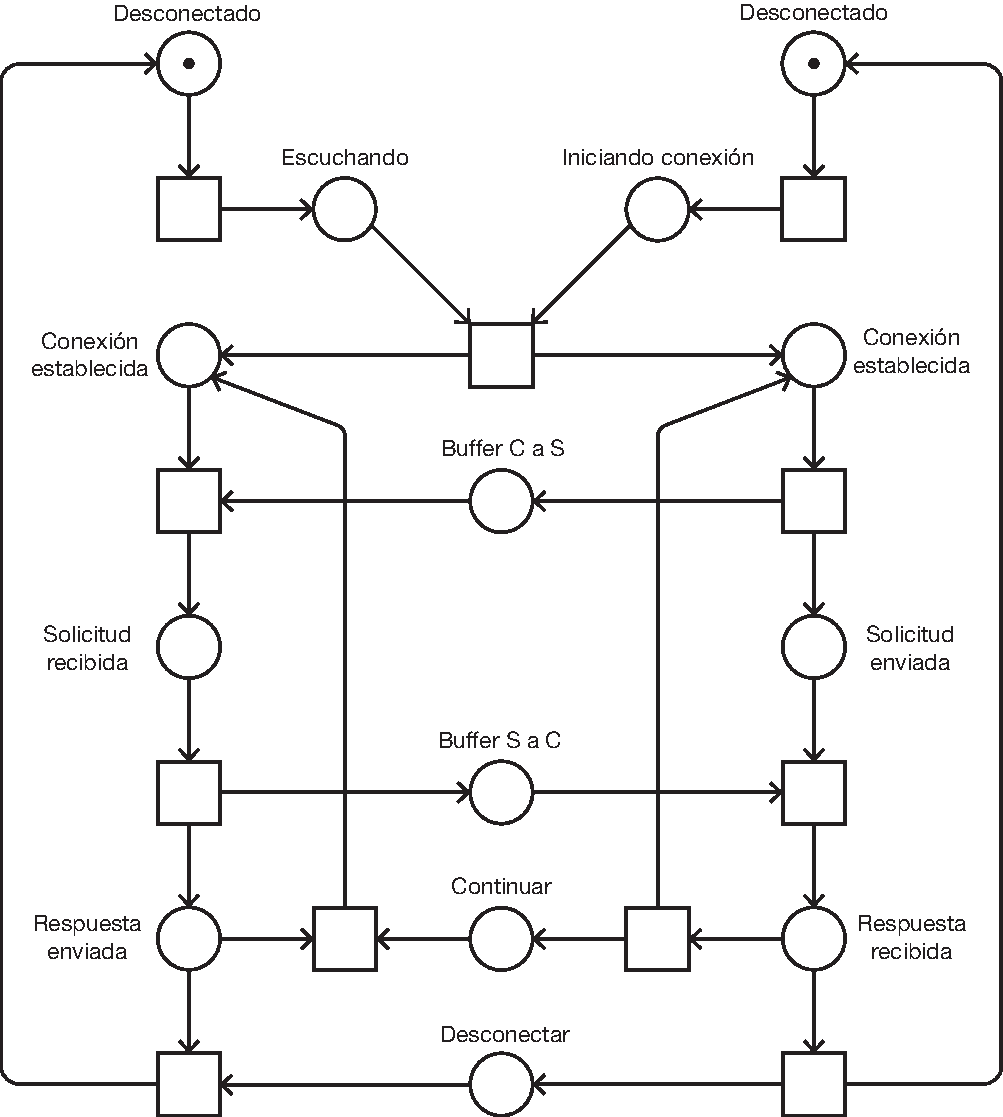
\includegraphics[width=0.8\linewidth]{imagenes/petri-net.pdf}
	\caption{Red de Petri modelando la interacción entre la aplicación de PC y el cartel.}
	\label{fig:petri-net}
\end{figure}

\subsection{Firmware}
El firmware del controlador del cartel es quien se encarga de aceptar pedidos de la aplicación de PC y ejecutar las acciones de cambio de mensaje, parámetros de animacion, configuración WiFi o de contraseña. Además, como se explicó en la sección \ref{sec:hw}, el ESP8266EX envía la configuración de las matrices de LED por serie.



\subsection{Plataformas de desarrollo}\label{sec:sdk}
El System on Chip ESP8266EX es muy popular y existen diversas formas de desarrollar para él, entre ellas están:
\begin{itemize}
	\item El SDK oficial \enquote{OS} de Espressif. Es un SDK privativo. Utiliza internamente FreeRTOS con lo que se puede programar con tareas y las primitivas de sincronización que FreeRTOS ofrece.
	\item El SDK oficial \enquote{NON-OS} de Espressif. Tiene \enquote{NON-OS} en su nombre porque con este SDK el programador no puede especificar ni crear tareas propias. Sino que se limita a registrar funciones callbacks que son llamadas por el firmware de Espressif cuando suceden eventos. La programación termina siendo basada en eventos.
	\item La implementación de la plataforma Arduino para el ESP8266EX. Es la más sencilla de utilizar. Tiene las mismas abstracciones que se utilizan en la plataforma Arduino original. Incluye clases C++ que implementan servidores HTTP y hay mucho software y soporte disponible.
\end{itemize}

Todas estas formas de desarrollar tienen en común que el software del programador corre sobre un firmware privativo, es decir, no es viable programarlo \enquote{bare-metal} porque los registros y todos la información del hardware necesario para realizar algo no trivial no está disponible.

Para el este proyecto se decidió utilizar el SDK \enquote{NON-OS}, donde las funciones que define el programador se ejecutan siempre enteramente, de forma cooperativa. Esto elimina toda una clase de problemas de interferencia de datos a causa de la concurrencia, con lo que no es necesario utilizar primitivas de sincronización.

Un ejemplo de esta técnica de programación se puede ver en la figura \ref{fig:callbacks}, donde se muestra como se registra la función que debe ejecutarse al recibir datos a través de una conexión TCP sobre 802.11. La aplicación llama a \code{espconn\_regist\_recvcb}, pasándole un puntero a función a \code{callback} y el firmware se encarga de llamar a \code{callback} cuando corresponda.

\begin{figure}[ht!]
	\begin{center}
		\centering
		\includegraphics[scale=0.8]{imagenes/callbacks.pdf}
		\caption{Ejemplo de uso de callbacks.}
		\label{fig:callbacks}
	\end{center}
\end{figure}



\subsubsection{Arquitectura general del programa}

El software que corre en el microcontrolador del cartel debe escuchar conexiones, y una vez establecida una conexión iniciada por la aplicación de PC, debe esperar a recibir un mensaje de autenticación con contraseña antes de permitir cambios del contenido del cartel.

Una vez que el usuario se autentica, el cartel espera un pedido de la aplicación de escritorio. Las interacciones posibles están descritas en mayor detalle en la sección \ref{sec:protocolo}.

El comportamiento del microcontrolador puede describirse como una máquina de estado finita jerárquica, como lo muestra la figura \ref{fig:fsm-micro}.

\begin{figure}[ht!]
	\begin{center}
		\centering
		\includegraphics[scale=0.8]{imagenes/fsm-micro.pdf}
		\caption{Máquina de estados finitos jerárquica del manejo de conexión en el microcontrolador.}
		\label{fig:fsm-micro}
	\end{center}
\end{figure}



\subsubsection{Requerimientos generales del programa embebido}

El programa que corre sobre el microcontrolador ESP8266 necesita conectarse a una red WiFi preexistente a fin de poder establecer una comunicación cifrada bajo el protocolo TLS con el cliente.
En esta sección, se hace referencia al cliente como la aplicación de PC.

El software debe actuar como servidor y manejar las peticiones que el cliente realice por medio de la aplicación de PC, detallada en la sección \ref{sec:pc}.
Dichas peticiones se clasifican en dos categorías: del tipo \enquote{get} y del tipo \enquote{get}. Las mismas se explican a continuación.

Las primeras corresponden a pedidos que solicitan información del sistema, mientras que las segundas permiten modificar dicha información.
Dentro de la categoría get, por un lado, el cliente puede loguearse en el sistema, obtener el texto que actualmente se muestra en el cartel, capturar la velocidad con la que se desplaza y con la que parpadea el contenido y pedir la configuración WiFi de la red a la que se encuentra conectado el microcontrolador.

A su vez, el cliente puede cambiar el contenido que desea representar, así como también modificar los parámetros relacionados a la velocidad de desplazamiento y parpadeo del texto.
Adicionalmente es posible modificar la configuración de la red a la que se autenticará la próxima vez que el ESP8266 se reinicie.
Por otra parte, el sistema posee una contraseña que es necesaria para realizar la acción de logueo.
Una vez logueado, dicha clave puede ser modificada. Estas acciones pertenecen a la categoría set.

Respecto de la información de la red, cabe destacar que los posibles parámetros que se pueden solicitar y cambiar son: el SSID, la contraseña WiFi, la dirección IP y la máscara de subred.

La figura \ref{fig:diagrama_casos_de_uso} muestra un diagrama de casos de uso, que describe todas las funcionalidades que el cliente puede realizar.
Adicionalmente, se observa como interactúan dichos pedidos, con el cartel.

\begin{figure}[!ht]
	\centering
	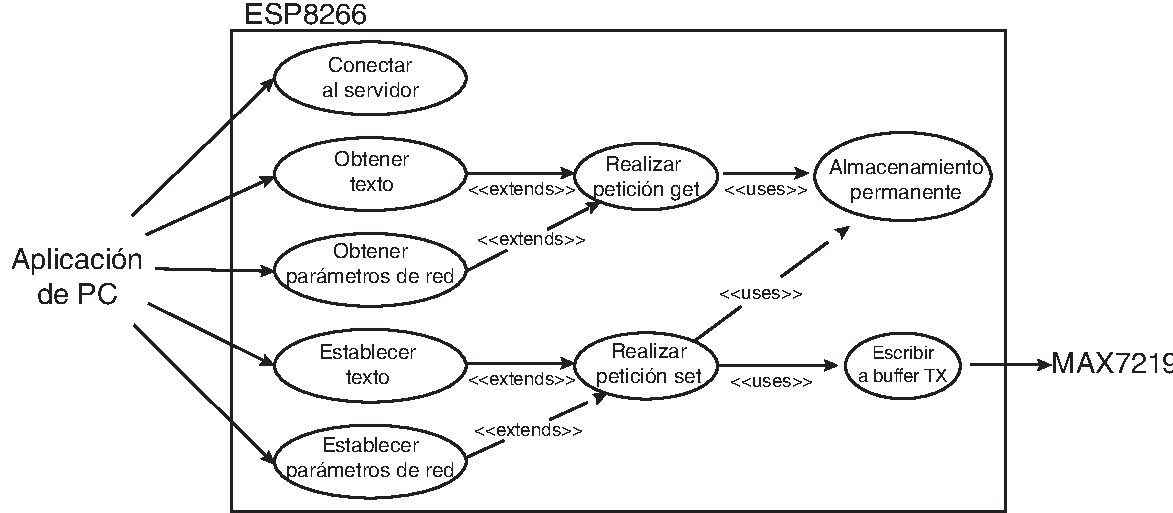
\includegraphics[width=1\linewidth]{imagenes/sistema-caso-de-uso.pdf}
	\caption{Diagrama de casos de usos.}
	\label{fig:diagrama_casos_de_uso}
\end{figure}

En la figura \ref{fig:diagrama_casos_de_uso} se observa, que entre las funcionalidades que el cliente realiza, se encuentra la de modificar los datos del cartel, tal como su contenido, su configuración WiFi y su contraseña del sistema.
Como el sistema puede, eventualmente, ser desprovisto de su alimentación o reseteado, es necesario que dichos cambios persistan aún cuando éstos eventos ocurren.

Por otra parte, el programa debe ser capaz de interpretar los pedidos que realiza el cliente y procesarlos a fin de generar la información que necesita el cartel para encender cada columna de luces.
Es necesario recordar que la matriz de LEDs está compuesta por módulos MAX7219 que son los encargados de recibir los datos enviados por el microcontrolador y encender las columnas de luces según corresponda.



\subsubsection{Secuencia de eventos del lado del microcontrolador}

En esta sección se enuncia brevemente, la secuencia de eventos que el usuario puede realizar con el sistema y cómo el programa responde ante los diferentes pedidos.
Es importante tener presente la figura \ref{fig:diagrama_casos_de_uso} donde se observa el diagrama de casos de uso que describe todas las funcionalidades que el cliente puede efectuar.

En primer lugar, el cartel se conecta a la red WiFi presentando las credenciales previamente almacenadas en la memoria no volátil del microcontrolador.
Esta acción es llevada a cabo gracias a una clase a nivel software denominada WiFiManager.
A su vez, el cliente accede a la aplicación de PC, con el ordenador conectado a la misma red.

El sistema le solicita la contraseña antes de realizar cualquier acción.
Una vez logueado, el cliente puede realizar cualquiera de las funcionalidades previamente enunciadas en la subsección anterior (tanto del tipo get como del tipo set).
Entre las acciones disponibles puede pedir información del texto que actualmente se encuentra representado en el cartel, o las credenciales de la red WiFi a la que el sistema se conecta.
Estas acciones, leen de la memoria no volátil del microcontrolador los datos necesarios y se la devuelven a la aplicación de PC.
El manejo de esta memoria persistente la realiza la clase conocida como Settings.

En caso de que el usuario desee modificar alguno de esos valores, puede hacerlo a través de la misma aplicación.
El mismo módulo de software que se encarga de leer de la memoria no volátil, obtiene los nuevos requerimientos que le provee el cliente, modifica sus variables internas y las almacena a fin de mantenerlas ante un futuro pedido.

El cartel, es decir el programa que corre sobre el microcontrolador, actúa de servidor atendiendo las peticiones que realiza el cliente de la aplicación de PC.
Esta funcionalidad es manejada por una clase de software denominada Server.
La misma es la encargada de recibir la cadena de bytes vía TCP y enviarla hacia el módulo MessageHandler.

En otras palabras MessageHandler toma la secuencia de bytes que le pasa la clase Server e interpreta esos datos utilizando el protocolo que se detalla en la sección \ref{sec:protocolo}.
Este protocolo ofrece soporte para interpretar cada acción que el cliente realiza ya que posee métodos para codificar y decodificar dichas peticiones.

MessageHandler decodifica los pedidos y los envía a la clase Settings o LedSign según pertenezcan a la cateogría de get o set respectivamente.
La clase Settings, ha sido enunciada previamente en esta sección, la misma se encarga de todos los pedidos que no requieran configurar la matriz de LEDs.
Mientras que LedSign obtiene los valores de configuración del tipo set y procesa los datos a fin de convertirlos en comandos que puedan ser interpretados por los dispositivos MAX7219, encargados de encender las luces del cartel.

En la figura \ref{fig:flujo_de_datos} se observa los distintos módulos de software previamente enunciados, y el intercambio de información que se realiza entre ellos.


\begin{figure}[!ht]
	\centering
	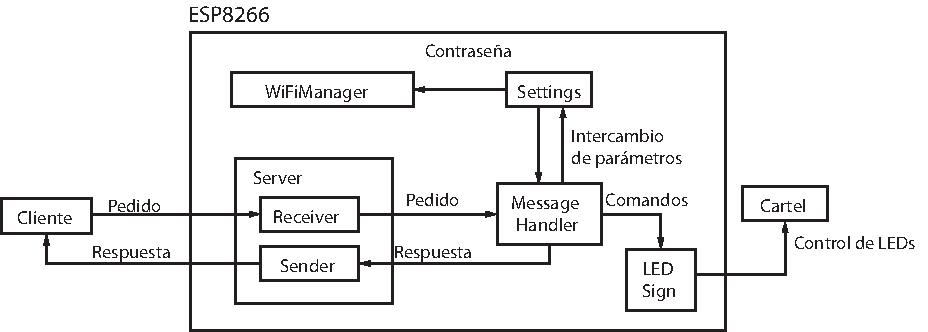
\includegraphics[width=1\linewidth]{imagenes/diagrama-bloque.pdf}
	\caption{Flujo de datos del lado del microcontrolador.}
	\label{fig:flujo_de_datos}
\end{figure}

A modo complementario se detalla un ejemplo relacionado a una secuencia de eventos que un cliente puede realizar.
En este caso, un usuario pide cambiar el texto que se muestra en la matriz. Este pedido es capturado por la clase Server quien le pasa la secuencia de bytes a MessageHandler.
Ésta interpreta la secuencia y obtiene el nuevo texto a representar. La información es enviada a LedSign quien desglosa el texto en letras y determina como deben encenderse las diferentes filas de la matriz de LEDs.
Por último, almacena el nuevo texto en la clase Settings para persistir la nueva información proporcionada.

A lo largo de esta sección se detalla cada clase mencionada, mostrando cuáles son sus interfaces de software y la forma en que se interconectan entre ellas.

\subsubsection{Archivo principal} \label{sec:archivo_principal}

\lstinputlisting[label=pseudo:userInit, linerange=1-10, firstnumber=1] {codigo/pseudocodigo/microcontrolador.pseudo}

El Archivo principal del programa que corre sobre el microcontrolador es el archivo main.cpp.
Dentro tiene un método denominado \code{user\_init()} que actúa como punto de entrada de la aplicación y no contiene parámetros.
En su definición se inicializa cada clase mencionada en la sección previa, ejecutando el método init( ) de cada una de ellas.
Dicho método es el encargado de asignar los valores iniciales a las variables internas de cada módulo de software, de forma de poder usar sus servicios públicos, posteriormente.
Éstas clases son las que se observan en la figura \ref{fig:flujo_de_datos}: WiFiManager, LedSign, Server y Settings.

Adicionalmente se establece tasa de bits por segundo a 115200 por medio de una función propia del SDK utilizado para el desarrollo.
Por último para utilizar los pines del micro, se inicializan los GPIO del microcontrolador, a través de la función gpio\_init( ) que también es propia del SDK.
En el fragmento \ref{pseudo:userInit} se muestra un pseudocódigo del método user\_init\( \).

Por último, se observa que para la clase Settings, se ejecuta el método loadSettings( ).
El mismo se encarga de cargar desde la memoria no volátil del microcontrolador, la última información almacenada respecto del texto a mostrar en el cartel, sus parámetros de configuración, y sus valores de red.


\subsubsection{Settings}

La clase Settings es la encargada de mantener en memoria RAM, la información principal respecto del cartel.
Entre ellas, contiene el texto a mostrar, su velocidad de parpadeo y desplazamiento y la información de la red a la que actualmente se encuentra conectado el sistema.
Además posee funcionalidades para almacenar dichos datos en memoria no volátil a fin de persistirlos ante un reinicio.
En la figura \ref{uml:settings}, se observa un diagrama UML con los principales métodos de la clase en cuestión, y a continuación se describe cada uno de ellos.

\begin{figure}[!ht]
	\centering
	\includegraphics[scale=0.8]{imagenes/uml/settings.pdf}
	\caption{UML de la clase Settings.}
	\label{uml:settings}
\end{figure}

\lstinputlisting[linerange=12-12, firstnumber=12] {codigo/pseudocodigo/microcontrolador.pseudo}

El método \code{init()} de settings se encarga de inicializar el puntero de la estructura de la flash de donde lee y almacena los datos.
Adicionalmente, la clase provee funcionalidad para establecer las configuraciones por defecto del sistema, presionando el botón de RST durante 5 segundos.
Para lograr eso, dentro del método \code{init()} también se inicializa el pin que se va a utilizar como reset (pin GPIO2) y se establece el callback para cuando dicho evento ocurra.
Se recomienda revisar la sección \ref{sec:sdk} donde se explica el mecanismo de callbacks que utiliza el microcontrolador.

\lstinputlisting[linerange=14-14, firstnumber=14] {codigo/pseudocodigo/microcontrolador.pseudo}

El método \code{loadSettings()} se encarga de cargar en memoria RAM la información necesaria del cartel utilizando el puntero previamente incializado en \code{init()}.
Adicionalmente se le envía, dicha información, a la clase LedSign quien es la encargada de mostrar el contenido anteriormente almacenado en la memoria.

En caso de que la información leída estuviese corrupta, la clase contiene un método privado para cargar los datos por defecto del sistema.
El método no posee parámetros.

\lstinputlisting[linerange=16-16, firstnumber=16] {codigo/pseudocodigo/microcontrolador.pseudo}

El método \code{storeSettings()} de la clase Settings provee funcionalidad para almacenar en la memoria no volátil la información actual del sistema.
Para la persistencia de los datos, se utiliza la librería propietaria del SDK denominada spi\_flash.h.
Este método no contiene parámetros.


\subsubsection{WiFiManager}

La clase WiFiManager es la encargada de administrar todas las configuraciones WiFi que necesita el microcontrolador para conectarse a una red.
Posee un sólo método público enunciado en el apartado \ref{sec:archivo_principal}, denominado init( ).

\lstinputlisting[linerange=18-18, firstnumber=18] {codigo/pseudocodigo/microcontrolador.pseudo}

El método no contiene parámetros y su principal tarea consiste en leer los datos de la clase Settings relacionados a la información de la red.
Dichos valores corresponden al SSID, contraseña de WiFi, ip, y máscara de subred y son utilizados para permitir al sistema conectarse a la red WiFi correspondiente.
La librería propia del SDK osapi.h permite realizar estas acciones.



\subsubsection{Server}

Una vez conectado a la red WiFi, la clase Server es la encargada de colocar al microcontrolador en modo servidor, de forma de poder atender las peticiones que realiza el usuario.
Provee funcionalidades para inicializar el servidor, desconectar la sesión, enviar mensajes hacia el cliente, y notificar cuando se recibe un paquete.
En el UML de la figura \ref{uml:server} se observan los métodos públicos de la clase que abstrae las funcionalidades mencionadas anteriormente.

\begin{figure}[!ht]
	\centering
	\includegraphics[scale=0.8]{imagenes/uml/server.pdf}
	\caption{UML de la clase Server.}
	\label{uml:server}
\end{figure}

Cabe destacar que en la figura \ref{uml:server} aparece una función privada relacionada a la recepción de mensajes denominada \code{receiveCallback()}.
Como bien su nombre lo indica, esto es un callback que se setea dentro del método \code{listen()} y se ejecuta cuando algún paquete llega al servidor (para más información, revisar la sección \ref{sec:sdk} donde se explica el método de callbacks).
A pesar de que sea un método privado, se decide mostrar en el UML debido a su reelevancia en esta solución.
Más adelanete, en esta sección, se explica su implementación.

\lstinputlisting[linerange=20-20, firstnumber=20] {codigo/pseudocodigo/microcontrolador.pseudo}

El método \code{init()} de la clase Server se ejecuta en el archivo principal y su función esencial consiste en inicializar las variables internas de la estructura de modo de permitir, posteriormente, colocar al microcontrolador en modo servidor.
Cabe aclarar que esta función debe ejecutarse después de haberse autenticado a una red WiFi; por ese motivo, primero se ejecta el \code{init()} de la clase WiFiManager.
Por otra parte, éste método no coloca al programa en modo servidor, es decir, no permite que distintos clientes se conecten todavía; para ello debe ejecutarse el método \code{listen()} que se describe a continuación.

\lstinputlisting[linerange=22-22, firstnumber=22] {codigo/pseudocodigo/microcontrolador.pseudo}

En primer lugar, el método \code{listen()} configura el certificado y la clave de seguridad del protocolo SSL que se utiliza en el intercambio de mensajes entre el servidor y el cliente de forma de que los mismos permanezcan cifrados hasta llegar a destino.
Adicionalmente, activa el mecanismo de Keep Alive propio de TCP, limita el número de conexiones simultáneas a uno y registrar los callbacks necesarios para su correcto funcionamiento (entre ellos el correspondiente a la recepción de paquetes).
El método no contiene parámetros.

\lstinputlisting[linerange=24-24, firstnumber=24] {codigo/pseudocodigo/microcontrolador.pseudo}

El método \code{send()} provee funcionalidad para enviar mediante TCP, hacia el cliente, un arreglo de bytes de manera cifrada.
Para su utilización, es necesario haber ejecutado el método \code{listen()} previamente y haber establecido una conexión con un cliente.

Recibe como parámetro un puntero que contiene la dirección del mensaje a enviar y el tamaño de dicho paquete.

\lstinputlisting[label=pseudo:receiveCallback, linerange=26-32, firstnumber=26] {codigo/pseudocodigo/microcontrolador.pseudo}

Como ya se mencionó anteriormente, el método \code{receiveCallback()} es una función privada que se ejecuta sólo cuando se reciben datos desde el cliente (size).
Contiene un buffer interno donde almacena los bytes que obtiene.
Los parámetros que recibe corresponden con la conexión vía TCP que envía los datos (conn), un puntero a la cadena de bytes recibido (data) y por último el tamaño de dicho arreglo.

Dicha estructura posee una capacidad limitada y, en este caso, su tamaño máximo se especifica en el protocolo de software (ver sección \ref{sec:protocolo}).
Cabe aclarar que la tarea de este método es acumular bytes hasta llenar el buffer. La clase Server no tiene las herramientas necesarias para interpretar la información que recibe.
Por ese motivo cuando la estructura se llena, se notifica a la clase MessageHandler quien es la que implementa el protocolo de comunicación diseñado para este proyecto y es quien es capaz de interpretar la secuencia de bytes recibida.



\subsubsection{MessageHandler}

La clase MessageHandler implementa el protocolo de comunicación entre el servidor y el cliente, y es capaz de interpretar el arreglo de bytes que recibe desde la clase Server.
Esta clase contiene un sólo método denominado \code{handle()} que atiende el mensaje que le envía el usuario y genera una respuesta para el cliente.
En el fragmento \ref{pseudo:messageHandlerHandle} se muestra un pseudocódigo del método a fin de brindar mayor claridad en la comprensión de la función.

\lstinputlisting[label=pseudo:messageHandlerHandle,linerange=36-93, firstnumber=36] {codigo/pseudocodigo/microcontrolador.pseudo}



\subsubsection{LedSign}

La última clase de la arquitectura del programa del microcontrolador es LedSign.
La misma se encarga de recibir los datos que envía MessageHandler por parámetro, procesarlos y armar un buffer de salida con la información necesaria para encender las luces de la matriz.
Cabe recordar que el programa del microcontrolador solo se comunica con el primer MAX7219 como lo indica la figura \ref{fig:flujo_de_datos}.
En la figura \ref{uml:ledSign} se muestra un UML con los métodos públicos que componen la clase.

\begin{figure}[!ht]
	\centering
	\includegraphics[scale=0.8]{imagenes/uml/LEDSign.pdf}
	\caption{UML de la clase LEDSign.}
	\label{uml:ledSign}
\end{figure}

\lstinputlisting[linerange=95-109, firstnumber=95] {codigo/pseudocodigo/microcontrolador.pseudo}

En primer lugar, el método \code{init()} se encarga de configurar los pines LATCH, CLK y DATA que se utilizan para la comunicación entre el microcontrolador y el MAX7219.
Para mayor información respecto de los pines, se sugiere visitar la sección \ref{sec:hw} %TODO poner la sección donde se explica los pines esos.

Adicionalmente se configura como salida los pines que se utilizan para los jumpers, se les habilita su pull up interno y se lee su valor a la salida.
De esta forma, se indica cuántos módulos de 8x8 LEDs componen el cartel.

Por otra parte, el método se encarga de configurar todos los registros necesarios de cada MAX7219 para iniciar su funcionamiento.
Entre las acciones que realiza, el programa se encarga de sacarlo del modo test, configurar la intensidad de los LEDs, indicarle que se van a usar las ocho columnas que posee el chip, limpiarle la pantalla apagando todos los LEDs y encenderlo.
Dichas configuraciones se realizan través del método \code{sendCommand()}.
La función toma dos parámetros, en el primero se especifica el registro a configurar y en el segundo el valor que se desea establecer.
Para más información respecto de la configuración de los registros consultar el datasheet del MAX7219 haciendo click en el siguiente \href{https://datasheets.maximintegrated.com/en/ds/MAX7219-MAX7221.pdf}{link}.

Finalmente se limpia el cartel, apagando todas las luces de cada módulo.

\lstinputlisting[linerange=111-111, firstnumber=111] {codigo/pseudocodigo/microcontrolador.pseudo}

El método \code{messageChanged()} se invoca cuando el mensaje o algún parámetro de configuración (tiempo de parpadeo o velocidad de desplazamiento) es modificado.

Recibe tres parámetros de configuración, el primero es el texto a mostrar.
Éste es un puntero a char donde se encuentra la información del contenido.
Es necesario que tenga un terminador nulo.
En caso de que no lo tenga, el comportamiento del método queda indefinido.

El segundo parámetro es brate, es un float que indica la velocidad de parpadeo que posee el texto.
Un valor negativo, repercute en comportamiento indefinido.
En caso de que no se requiera se debe colocar un 0.

El último parámetro es srate que también es un float que indica la velocidad a la que se desplaza el contenido.
La diferencia con el anterior radica en que este sí puede tomar valores negativos.
Un valor negativo indica que el contenido se desplaza a la izquierda, mientras que un positivo lo hace hacia la derecha.
En caso de que no se requiera el uso de esta funcionalidad, se debe colocar un 0. 

La función principal de este método es tomar los datos de configuración que se reciben por parámetro y armar un buffer de salida con la información de cada columna del cartel, respecto del estado de cada LED.
Para realizar el desplazamineto del contenido, la estrategia que se adopta es periódicamente, mover el índice del buffer y enviar nuevamente la información al MAX7219.
Para el tiempo se utiliza una estructura propia del SDK del microcontrolador denominado timer\_t.
La misma permite ejecutar un callback cuando se cumple un determinado lapso de tiempo.

Para realizar el parpadeo del mensaje, se adopta una estrategia similar.
Basándose en otro timer\_t se envía periódicamente un comando a cada MAX7219 que le indica que debe encenderse o apagarse, según corresponda.


\subsection{Aplicación de PC}\label{sec:pc}
La aplicación de PC es un programa con interfaz gráfica que permite al usuario administrar el contenido y configuración del cartel de forma remota. En el marco del protocolo definido en el \ref{sec:protocolo}, la aplicación de PC es el cliente.

\subsubsection{Plataforma de desarrollo}
La aplicación está desarrollada en el \emph{framework} de desarrollo Qt. Qt es un conjunto muy amplio de librerías que permiten el desarrollo de aplicaciones gráficas que se pueden compilar para distintas plataformas (Windows, GNU/Linux, macOS o cualquier variante de Unix con X11). El lenguaje de programación que se utiliza es C++ con extensiones propias de Qt.

\subsubsection{Arquitectura basada en eventos}\label{sec:qt}
Qt permite desarrollar aplicaciones con una arquitectura basada en eventos. Sin embargo, la implementación de este sistema de eventos no está basada en los mecanismos más clásicos como el patrón Observer de la programación orientada a objetos ni el mecanismo de callbacks o punteros a funciones propios de la programación procedural, sino que hay métodos en los objetos que pueden ser denominados \emph{signals} o \emph{slots}.

Una clase puede tener opcionalmente uno o más métodos que sean \emph{signal} o \emph{slot}. La idea clave de estas sistema es que un objeto puede \enquote{emitir} una \emph{signal} que ejecuta el método \emph{slot} de otro objeto (o incluso posiblemente el mismo emisor) al cual se estableció previamente lo que se denomina \enquote{conexión}. Se ilustra este mecanismo en la figura \ref{fig:signals-slots}

\begin{figure}[!ht]
	\centering
	\includegraphics[height=8cm]{imagenes/signal-slots.png}
	\caption{Mecanismo de \emph{signal} y \emph{slot}.}
	\label{fig:signals-slots}
\end{figure}

En Qt, las clases que necesiten utilizar el sistema de eventos deben heredar de una clase provista por la librería llamada \code{QObject}. Esta clase provee distintas funcionalidades al resto de las clases definidas por Qt. Entre los objetos que heredan de QObject puede existir una relación de parentesco, en la cual un objeto $B$ puede tener como padre a otro objeto $A$. Esto, por ejemplo, sirve para liberar al programador del manejo de memoria: un objeto puede destruir a sus hijos antes de destruirse a sí mismo (por destrucción se entiende la liberación de todo recurso asociado al objeto, como memoria o archivos).

El mecanismo de \emph{signal} y \emph{slots} tiene como una de sus ventajas el hecho de que la ejecución de un \emph{slot} darse en otro hilo. Esto esta relacionado con la idea que promueve Qt de que un objeto puede \enquote{pertenecer} a un hilo de ejecución (encapsulado por la clase \code{QThread}), esto permite que no haya interferencia de datos causada por la concurrencia ya que no hay accesos explícitos a variables compartidas entre hilos sino que pueden enviar datos como argumentos a los \emph{slots}, de forma similar al paradigma de pasaje de mensajes en programación concurrentes.

Por ejemplo, en el caso del objeto \code{Object1} en la figura \ref{fig:signals-slots}, en algún método suyo se podría tener código como el siguiente:
\begin{lstlisting}[language=c++]
	// ...
	emit signal1();
	// ...
\end{lstlisting}

Mientras que \code{Object2} tiene un \emph{slot} llamado \code{slot1()} al cual \code{signal1()} de \code{Object1} está conectado. Entonces al emitirse \code{signal1()}, se ejecuta también \code{slot1} de \code{Object2} (además de los otros métodos pertenecientes a las otras clases que aparecen en la figura).

El momento en que se ejecuta un \emph{slot} depende del tipo de conexión que se haya establecido entre los objetos. Qt define tres tipos de conexiones:
\begin{description}
	\item[\code{DirectConnection}:] el \emph{slot} se ejecuta en el mismo hilo de ejecución desde el cual se hizo la emisión. Esto es útil para cuando los objetos que están conectados pertenecen a un mismo hilo o también cuando pertenecen a distintos hilos pero se toma precaución utilizando primitivas de sincronización para serializar el acceso al recurso o memoria compartida.
	\item[\code{QueuedConnection}:] se coloca un pedido de ejecución de \emph{slot} (con los argumentos que se hayan emitido) en la cola de eventos del hilo del objeto destino. Esto es lo que libera al programador de tener que utilizar primitivas de sincronización explícitas y es lo que se usa mayormente en la aplicación de PC de este proyecto. La ejecución de \code{emit} retorna inmediatamente, con lo que el hilo del objeto emisor no se bloquea al emitir una señal.
	\item[\code{BlockingQueuedConnection}:] Similar a \code{QueuedConnection}, con la diferencia que el hilo emisor se bloquea hasta que finalice la ejecución de los \emph{slots} que haya activado. Si no se utiliza con precaución y se establecen conexiones cíclicas, existe el riesgo de que ocurra un \emph{deadlock}, ocurrencia en la que un conjunto de hilos se espera entre sí indefinidamente, deteniendo parcial o íntegramente el programa.
\end{description}

Internamente, la implementación de Qt tiene una cola bloqueante de eventos para cada uno de los hilos que tengan una instancia de la clase \code{QThread}. También lleva registro de cuáles objetos que heredan de \code{QObject} pertenecen a cuál hilo. De esta manera, la ejecución de un hilo consiste principalmente en esperar a que hayan eventos para procesar en una cola bloqueante, cuya implementación específica depende de la plataforma para la cual se esté compilando el programa.

\subsubsection{Módulos}
En esta sección se listan las clases más relevantes de la aplicación de PC, sus métodos públicos principales y la interacción entre ellos.
Las clases son:
\begin{description}
	\item[\code{Panel}:] Provee la interfaz gráfica principal, que consiste en una ventana con los distintos elementos de control para que el usuario pueda manipular el cartel. Se puede ver una captura de pantalla en la figura \ref{fig:panel-screenshot}.
	\item[\code{Client}:] Realiza la interacción con el cartel a nivel mensaje del protocolo. Se encarga de generar los mensajes salientes y de tomar las acciones pertinentes ante una respuesta del cartel (servidor). La (única) instancia de esta clase \enquote{pertenece} (ver sección \ref{sec:qt}) a otro hilo en el cual se realizan todas las operaciones bloqueantes de entrada y salida, de forma que no se bloquea el hilo principal, que causaría que la interfaz gráfica deje de responder a eventos del sistema o del usuario.
	\item[\code{Connection}:] Abstrae la conexión al cartel, exponiendo métodos que envían y reciben específicamente los mensajes definidos en el protocolo. En esta clase también se hace la carga del certificado TLS antes de establecer una conexión.
	\item[\code{SignModel}:] Una clase \enquote{tonta} que agrupa todos los parámetros modificables del cartel, como el texto del cartel y sus parámetros de animación, los datos de la red Wifi a la que se debe conectar el cartel, etc. Existe principalmente para llevar registro de cuales parámetros fueron cambiados por el usuario y ameritan un pedido de cambio hacia el cartel. De manera que no se hagan cambios innecesarios al contenido o configuración del cartel.
\end{description}

Se puede ver en la figura \ref{fig:uml-cliente} un diagrama de los objetos mencionados anteriormente. No están incluidas las conexiones entre los objetos para mantener la prolijidad del diagrama.

Los objetos están repartidos entre los dos hilos como se muestra en la figura \ref{fig:qt-threads}.

\begin{figure}[!ht]
	\centering
	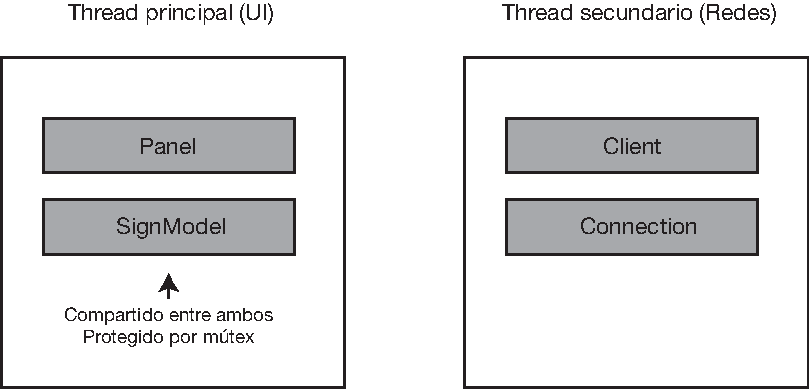
\includegraphics[scale=0.8]{imagenes/qt-threads.pdf}
	\caption{Distribución de los objetos en hilos.}
	\label{fig:qt-threads}
\end{figure}

\begin{figure}[!ht]
	\centering
	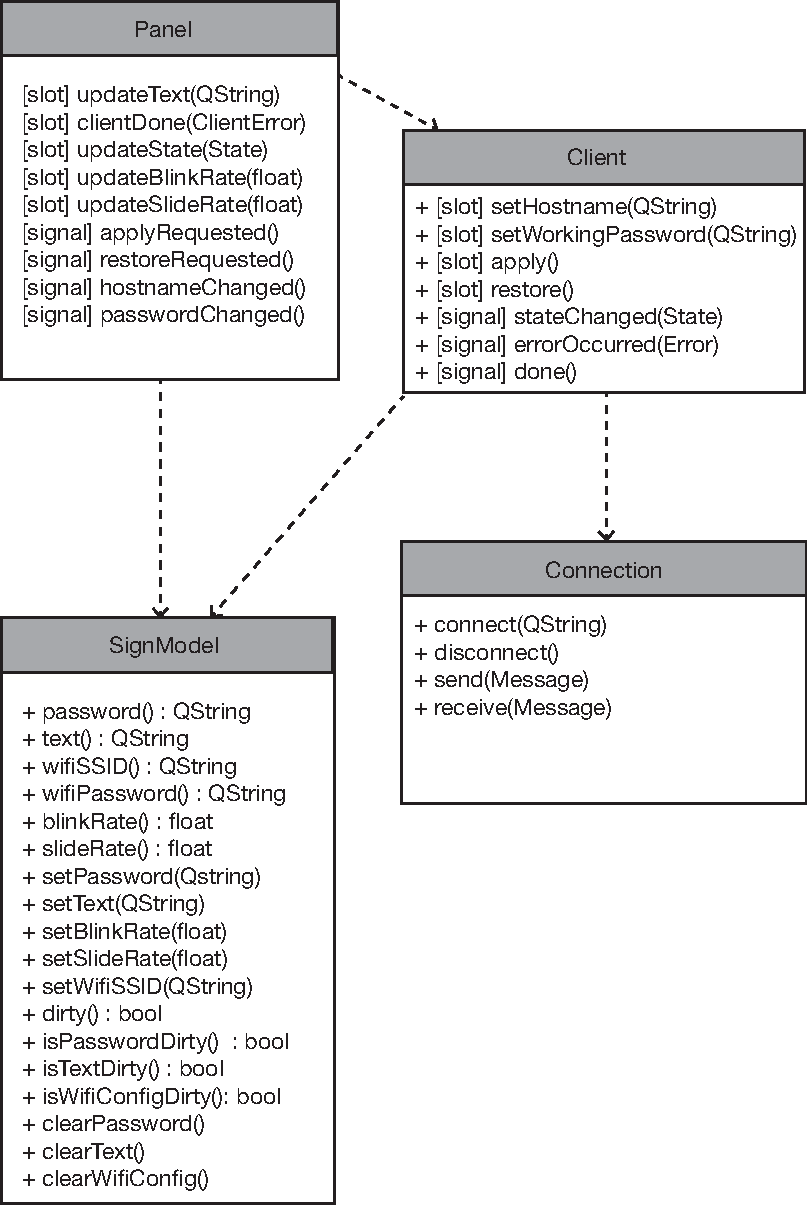
\includegraphics[scale=0.8]{imagenes/uml-cliente.pdf}
	\caption{Diagrama UML de las clases más relevantes.}
	\label{fig:uml-cliente}
\end{figure}

\begin{figure}[!ht]
	\centering
	\includegraphics[height=10cm]{imagenes/panel-screenshot.png}
	\caption{Captura de pantalla de la ventana principal de la aplicación de pc.}
	\label{fig:panel-screenshot}
\end{figure}

\paragraph{Panel}
La clase Panel implementa la interfaz gráfica mediante la cual el usuario ingresa y visualiza el contenido y configuración del cartel. Sus métodos no deben hacer operaciones que tarden, ya que eso resultaría en que la interfaz de usuario se congele. Por esto y para lograr una mejor separación de propósito en las clases, la clase Panel solo se encarga de este aspecto del programa.

Un flujo típico de ejecución es el siguiente:
\begin{enumerate}
	\item La clase se inicializa a su misma y sus objetos asociados (entre ellos, una instancia de Client y una de SignModel).
	\item Se muestra el diálogo en el cual se ingresa la dirección de IP o nombre de host del cartel a cual conectarse. Ver figura \ref{fig:login}
	\item Asumiendo que no se seleccionó \enquote{Cancelar} en el diálogo anterior, el objeto Panel inicia una interacción para traer el estado (contenido y configuración) del cartel. Hace esto emitiendo la señal \code{restoreRequested()}, que está conectada al \emph{slot} \code{apply()} del objeto de clase Client.
	\item El objeto de tipo Panel desactiva todos los elementos de la interfaz gráfica de forma que no se pueda realizar otra operación mientras haya una interacción en curso.
	\item El objeto de tipo Panel continúa procesando los eventos de la cola de eventos normalmente. Uno de estos eventos será una señal \code{done(ClientError)} de Client, conectada al \emph{slot} \code{clientDone(ClientError)} de Panel. El argumento es un enumerativo que representa un error o éxito. También, durante el transcurso de una interacción, Client va emitiendo señales para notificar de cambios de su estado interno, para poder mostrar mensajes al usuario sobre la fase de la interacción actual (\enquote{Conectando},\enquote{Esperando respuesta...}, etc).
\end{enumerate}

\begin{figure}[hbtp]
	\centering
	\includegraphics[scale=0.8]{imagenes/login.png}
	\caption{Captura de pantalla de la ventana de login.}
	\label{fig:login}
\end{figure}

\paragraph{Client}
Client es la clase que implementa la interacción en si a nivel mensajes de protocolo. Es decir, es la clase que sabe qué mensajes emitir y que hacer ante las respuestas.

Cuando se inicia una interacción del tipo \enquote{get}, simplemente inicia una conexión (utilizando un objeto de tipo Connection), y realiza dos interacciones en la misma conexión: una para traer el contenido del cartel y otra para traer la configuración de WiFi.

Por otro lado, cuando se inicia una interacción del tipo \enquote{set}, debe primero determinar cuales partes del módelo del cartel han cambiado y deben, por ende, ser actualizadas. Para eso usa unos métodos de SignModel que permiten cuales datos han sido cambiados por el usuario. Estos son: \code{isPasswordDirty()}, \code{isTextDirty()} y \code{isWifiConfigDirty()}.

A lo largo de una interacción, el objeto de tipo Client va cambiando de estados. Internamente tiene un enumerativo con los siguientes valores:
\begin{description}
	\item[Disconnected:] Client está listo para iniciar una interacción.
	\item[Connecting:] Se envió una solicitud de conexión y se está esperando una respuesta.
	\item[Connected:] Se recibió una respuesta a la solicitud de conexión y hay una conexión establecida.
	\item[RequestSent:] Se envió un pedido (ver sección \ref{sec:protocolo}) y se espera una respuesta.
	\item[ResponseReceived:] Se recibió una respuesta y se está procesándola.
\end{description}

Los estados Connected y ResponseReceived existen más bien por completitud, ya que el tiempo en que se permanece en esos estados no es perceptible.

También se define en esta clase un enumerativo \code{ClientError}, que representan los distintos errores en los que puede finalizar una interacción. Tiene los siguientes valores:
\begin{description}
	\item[Ok:] La interacción fue exitosa.
	\item[CertificateMissing:] No se pudo cargar el certificado TLS.
	\item[Timeout:] Se excedió el tiempo de espera a una respuesta.
	\item[WrongResponse:] Se recibió una respuesta incorrecta por parte del servidor. Esto puede suceder si hay un error en la implementación del protocolo, o si a lo que se conectó no es un cartel, sino algun otro servicio sobre TLS, como un servidor web con HTTPS.
	\item[IncompleteWrite:] No se pudo mandar un mensaje entero. Se debe a un problema externo de red.
	\item[ConnectionRefused:] El host remoto rechazó la conexión. Muy posiblemente no sea un cartel.
	\item[RemoteHostClosed:] El host remoto cerró inesperadamente la conexión. Esto puede pasar si alguna fase de la interacción tardo demasiado (por congestión de la red, por ejemplo), haciendo que el cartel cierre la conexión.
	\item[HostNotFound:] No se pudo resolver la dirección IP del nombre de host dado.
	\item[NetworkError:] Error de red genérico.
	\item[SslHandshakeFailed:] Falló el establecimiento de una conexión TLS. Esto puede darse por certificados y claves que no coinciden, corrupción de ellos o un error en la implementación de TLS del ESP8266EX.
	\item[SslInternalError:] Error interno de OpenSSL (librería que maneja las conexiones TLS).
	\item[SslInvalidData:] El certificado público cargado no es válido.
	\item[Unknown:] Error desconocido genérico.
	\item[ServerMalformedPacket:] Se recibió un paquete no conforme a lo descrito por la especificación del protocolo.
	\item[ServerBadPassword:] Se trató de iniciar una interacción con una contraseña incorrecta.
	\item[ServerBadProtocolVersion:] El cartel tiene una versión del protocolo más nueva que la de la aplicación de PC.
\end{description}
\paragraph{Connection}
Esta clase es más pequeña que las anteriores. Provee una interfaz simple para iniciar una conexión TLS y mandar mensajes. Tiene los siguientes métodos bloqueantes:
\begin{description}
	\item[\code{bool connect(const QString hostname)}:] Inicia una conexión TLS al host con nombre dado por \code{hostname}. Retorna falso si hubo error o timeout.
	\item[\code{bool disconnect()}:] Cierra la conexión. Es idempotente: si no existía previamente una conexión abierta, no realiza ninguna acción.
	\item[\code{bool send(const Message \&msg)}:] Envia el mensaje \code{msg}. Retorna falso si hay error o timeout.
	\item[\code{bool receive(Message \&msg)}:] Recibe un mensaje y lo almacena en \code{msg}. Retorna falso si hay error o timeout.
	\item[\code{QAbstractSocket::SocketError lastError()}:] Retorna un enumerativo con el último error de red. Este enumerativo es propio de Qt y luego se mapea a un valor del enumerativo \code{Client::ClientError}.
\end{description}

Todos estos métodos tienen un tiempo de expiración o \emph{timeout} definido por la constante estática \code{Connection::TIMEOUT\_MS}

\subsection{Protocolo de comunicación} \label{sec:protocolo}

\subsubsection{Codificación}

Cada mensaje del protocolo es un paquete de tamaño fijo de tamaño igual a 256 bytes.
Dentro de esa longitud está incluido el header.
Todos los valores numéricos se transmiten con orden de bytes Big-Endian.
Cada mensaje respeta un formato base común. Se puede ver este formato en la figura \ref{fig:paquete-base}.


\begin{figure}[!ht]
	\centering
	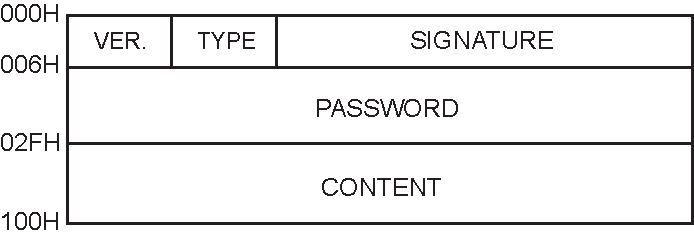
\includegraphics[width=0.6\linewidth]{imagenes/protocolo/paquete-base.pdf}
	\caption{Esquema general entre todos los componentes del sistema.}
	\label{fig:paquete-base}
\end{figure}

\begin{itemize}
	\item version: es un número de 8 bits que identifica la versión del protocolo, por si se hicieran cambios y se quiera mantener retrocompatibilidad.
	\item type: es un enumerativo que codifica el tipo de mensaje. Más adelante se detalla los diferentes tipos posibles.
	\item signature: es una palabra de 4 caracteres que siempre tiene que ser ANRS.
	\item password: es la contraseña del sistema. Debe incluirse en cada paquete que se envía hacia el microcontrolador. Los paquetes que envía éste como respuesta dejan dicho campo vacío.
	\item content: es una estructura cuya interpretación depende de type y se define más adelante.
\end{itemize}



\subsubsection{Interacción}

El primer paso para comenzar una interacción debe hacerla el cliente, iniciando una conexión TLS con el servidor.
A continuación, el usuario envía un mensaje denominado request y que puede tomar alguno de los siguiente valores en su campo type.

\begin{itemize}
	\item SetPassword: establece una nueva contraseña del sistema.
	\item GetText: pide, al servidor, el contenido del cartel, su velocidad de parpadeo y desplazamiento.
	\item SetText: establece el nuevo contenido del cartel, su velocidad de parpadeo y desplazamiento.
	\item GetWiFiConfig: pide, al servidor, la configuración WiFi relacionada a la red a la que actualmente se encuentra conectado el microcontrolador.
	\item SetWiFiConfig: establece la nueva configuración WiFi respecto de la nueva red a la que el microcontrolador debe conectarse la próxima vez que se inicie el sistema.
\end{itemize}

Así mismo, el cliente, debe especificar la versión de protocolo que utiliza, la firma y la contraseña del sistema.
Por su parte, el servidor, recibe el paquete, analiza todos los campos del header y emite una respuesta hacia el cliente de acuerdo al pedido realizado por éste.
El campo type de la respuesta puede obtener los siguientes valores.

\begin{itemize}
	\item GetTextResponse: envia hacia el usuario la información del contenido y los parámetros de configuración del cartel.
	\item GetWiFiConfigResponse: envia hacia el usuario la información respecto de la red WiFi a la que actualmente se encuentra conectado el servidor.
	\item GenericResponse: es un tipo de paquete que se envía de vuelta, cuando alguno de los datos proporcionados por el cliente no son válido.
\end{itemize}

Respecto de este último tipo de mensajes, los códigos de respuesta posibles son los que se listan a continuación.

\begin{itemize}
	\item OK: se envía ante un pedido de cambio de algún parámetro enunciado previamente, cuando la operación fue realizada satisfactoriamente.
	\item MalformedPacket: se envía cuando el paquete recibido de parte del cliente contiene una firma o un tipo inválido.
	\item BadPassword: se envía cuando la contraseña proporcionada por parte del cliente es incorrecta.
	\item BadProtocolVersion: se envía cuando el protocolo del programa es superior al que soporta el servidor.
	\item BadIP: se envía cuando la nueva ip proporcionada es incorrecta.
	\item BadSubnetMask: se envía cuando la nueva máscara de red proporcionada es incorrecta.
\end{itemize}

Luego de obtener la respuesta, el cliente debe cerrar la conexión inmediatamente.
De esta forma se completa una interacción entre el usuario y servidor.
En caso de que la conexión no fuera cerrada por el usuario, el servidor pasado un cierto tiempo la finaliza.
A lo largo de esta sección se detallan las distintas estructuras del campo content, de forma de mostrar a qué corresponde cada campo.



\subsubsection{SetPassword}

El paquete de este tipo permie cambiar la contraseña del sistema.
En content se encuentra la nueva contraseña, tiene un máximo de 40 caracteres sin incluir al caracter nulo.
La respuesta que se recibe es del tipo GenericResponse.



\subsubsection{GetText}

El paquete de este tipo permite obtener el contenido actual del cartel, así como también sus configuraciones relacionadas a la velocidad de parpadeo y desplazamiento del mensaje.
El campo content queda vacío puesto que su contenido no es utilizado para procesar la petición.

Se espera una respuesta del servidor del tipo GetTextResponse donde el contenido posee toda la información previamente mencionada.



\subsubsection{SetText}

El paquete de este tipo permite establecer un nuevo mensaje a representar en el cartel, así como también sus parámetros de configuración.
El campo content debe respetar la estructura que se observa en la figura \ref{fig:paquete-anim}


\begin{figure}[!ht]
	\centering
	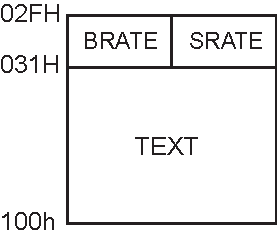
\includegraphics[width=0.3\linewidth]{imagenes/protocolo/paquete-anim.pdf}
	\caption{Esquema general entre todos los componentes del sistema.}
	\label{fig:paquete-anim}
\end{figure}

BRATE y SRATE son la frequencia de parpadeo en Hz y la velocidad de deslizamiento en píxeles por segundo.
Se asume que si BRATE es cero, no se debe parpadear el contenido.
De la misma forma, si SRATE es cero, no se debe deslizar el contenido.
El tipo de dato ufp844 es un número en punto fijo sin signo con 4 bits de parte entera y 4 bits de parte fraccionaria.
El tipo de dato sfp844 es lo mismo que ufp844 pero en complemento a dos.
Por último, en content se encuentra el campo text asociado al mensaje a mostrar en el cartel.
El mismo debe tener un terminador nulo para indicar el fin del contenido.
La respuesta que se recibe es del tipo GenericResponse.



\subsubsection{GetWiFiConfig}

El paquete de este tipo permite obtener el SSID, contraseña WiFi, ip y máscara de subred respecto de la red a la que actualmente se encuentra cnectado el servidor.
El campo content queda vacío puesto que su contenido no es utilizado para procesar la petición.

Se espera una respuesta del servidor del tipo GetWiFiConfigResponse donde el contenido posee toda la información previamente mencionada.



\subsubsection{SetWiFiConfig}

El paquete de este tipo permite establecer un nuevo SSID, contraseña WiFi, ip y máscara subred respeco de la red que se conectará la próxima vez que se incie el sistema.
El campo content debe respetar la estructura que se observa en la figura \ref{fig:paquete-wifi}


\begin{figure}[!ht]
	\centering
	\includegraphics[width=0.5\linewidth]{imagenes/protocolo/paquete-wifi.pdf}
	\caption{Esquema general entre todos los componentes del sistema.}
	\label{fig:paquete-wifi}
\end{figure}

La respuesta que se recibe es del tipo GenericResponse.


\subsubsection{Strings}

Los strings tienen un límite de longitud dado por el lugar remanente en el mensaje y están codificados según el estándar ISO/IEC 8859-1:1998.
El último byte del contenido, es necesario colocar un caracter nulo de modo que indique el final de la cadena de texto.


\subsubsection{Transport Layer Security}\label{sec:tls}